%! Author = mateusz
%! Date = 20/09/2025

\chapter{Prezentacja systemu}
\label{ch:prezentacja-systemu}

W niniejszym rozdziale przedstawiono końcowy wygląd aplikacji oraz opisano sposób korzystania
z jej kluczowych funkcjonalności.
Opis obejmuje zarówno widoki dostępne publicznie, jak i elementy wymagające uwierzytelnienia użytkownika.

%! Author = Mateusz
%! Date = 13/11/2025

\subsection{Strona główna}
\label{subsec:strona-glowna-frontend}

Jednym z głównych modółów aplikacji jest strona główna.
Pełni ona rolę głównej wyszukiwarki spotów, dzięki której użytkownik może w
łatwy sposób znaleść interesujące go lokacje.
Posiadan ona dwa tryby prosty i zaawansowany, dzięki przyciskowi na samej górze strnony można się łatwo
przełączyć między tymi widokami.
Na prostym znajduje się karuzela z 12 najpopularniejszymi spotami w całej aplikacji, użytkownik może tutaj
wyszukać spoty po lokalizacji ( kraj, region, miasto).
Na zaawansowanym widoku jest wyszukiwarka która filtruje po mieście, tagach oraz ocenie dodatkowo
sortuje po popularności i ocenach.

Strona główna została zbudowana z dwóch głównych komponentów HomePaga oraz AdvanceHomePage.
W skład prostej wersji wchodzą następujące komponenty:
\begin{itemize}
  \item Switch - służy do przełączania widoku między trybem podstawowym a zaawansowanym
  \item SearchBar - wyszukiwarka spotów
  \item Carousel - wyświetla najpopularnejsze spoty
  \item SearchSpotList - wyświetla wyszukane spoty
\end{itemize}

W skład zaawansowanej wersji wchodzą następujące komponenty:
\begin{itemize}
    \item Switch - służy do przełączania widoku między trybem podstawowym a zaawansowanym
    \item AdvanceSearchBar - wyszukiwarka spotów
    \item SearchSpotList - wyświetla wyszukane spoty
\end{itemize}

Komponent Switch zawiera w sobie dwa NavLink z biblioteki React Router dzięki temu można przełącznyć widok bez niepotrzebnych
odświeżeń strony.

W koponencie SearchBar po wpisaniu conajmniej 2 znaków pojawi się lista z podpowiedziami
do kraju, regionu oraz miasta w zależności od tego które aktualnie uzupełniamy.
Po pokazaniu się tej listy można wybrać interesujące nas miejsce dzięki czemu
wiemy w jakich lokalizacjach znajdują się spoty.

SearchSpotList zawiera listę komponentów SpotTile, LoadingSpiner oraz komunikat który
wyświetli się jeżeli nie zostanie wyświetlony żaden spot.

Spot tile zawiera informacje takie jak:
\begin{itemize}
    \item Zdjęcie spota
    \item Miasto w którym  się znajduje
    \item Nazwę
    \item Oceny i ich liczbę
    \item Tagi
    \item Podstawowe informacje pogodowe (temperatura i typ)
    \item Dwa przyciski, jeden do przejścia do szczegółów a drugi z informacją jak daleko znajduje
    się dany spot, po kliknięciu pokazuje go na mapie.
\end{itemize}

Komponent AdvanceSearchBar wygląda bardzo podobnie tylko z lokalizacji można podać tylko miasto,
dodatko jest mozżliwość dodania tagów z listy.
Jest też filtrowanie po ocenie oraz sortowanie po ocenie i popularności (komponenty Dropdown).

%\begin{figure}[H]
%    \centering
%    \includegraphics[width=1\textwidth]{attachments/implementacja-strona-glowna1}
%    \caption{Implementacja strony głównej}
%    \label{img:implementacja-strona-glowna1}
%\end{figure}
\subimport{chapters/prezentacja-systemu/sections/}{strona-glowna.tex}
\subimport{chapters/prezentacja-systemu/sections/}{strona-mapy.tex}
\subimport{chapters/prezentacja-systemu/sections/}{strona-chatu.tex}
\subimport{chapters/prezentacja-systemu/sections/}{strona-forum.tex}
%! Author = mateusz
%! Date = 20/10/2025

\subsection{Panel logowania}
\label{subsec:panel-logowania-frontend}

\subimport{chapters/prezentacja-systemu/sections/}{panel-konta-uzytkownika.tex}
%! Author = Mateusz
%! Date = 19/12/2025

\subsection{Sidebar}
\label{subsec:sidebar-frontend}

\glslink{sidebar}{Sidebar} stanowi główny komponent nawigacyjny aplikacji.
Implementacja obejmuje:
\begin{itemize}
    \item zestaw komponentów interfejsu odpowiedzialnych za renderowanie pozycji, podmenu, tooltipów oraz obsługę
    interakcji użytkownika,
    \item pliki pomocnicze służące do budowania listy linków i rozpoznawania typów elementów nawigacji
    (\texttt{functions}, \texttt{sidebarLinks}),
    \item definicje typów i interfejsów opisujących strukturę pozycji paska bocznego (\texttt{link}),
    \item moduł \texttt{Redux} przechowujący stan rozwinięcia paska (\texttt{sidebar.ts}).
\end{itemize}

\subsubsection{Komponenty}

\textbf{\texttt{Sidebar}} \\
Komponent odpowiada za złożenie całej nawigacji oraz sterowanie jej zachowaniem.
Wykorzystywane są \glslink{hook}{hooki} \texttt{useDarkMode} (obsługa motywu), \newline \texttt{useSelectorTyped}
(odczyt \texttt{isLogged} oraz \texttt{isSidebarOpen}) oraz \texttt{useLocation} (sprawdzenie aktualnej ścieżki).
Na podstawie lokalizacji ustalany jest tryb pozycjonowania: dla stron o układzie „sticky”
(panel użytkownika, czat, strona główna) stosowana jest klasa \texttt{xl:sticky}, w pozostałych przypadkach \texttt{absolute}.
Zestawy linków nawigacyjnych budowane są w pliku \texttt{sidebarLinks} (opis w podrozdz. \ref{subsubsec:sidebar-links-files}).

W strukturze komponentu renderowane są:
\begin{itemize}
    \item \texttt{SidebarToggleButton},
    \item sekcja nawigacyjna: \texttt{SidebarSection} $\rightarrow$ \texttt{SidebarList} (linki główne),
    \item sekcja opcji: \texttt{SidebarSection} $\rightarrow$ \texttt{SidebarList} (akcje i opcje).
\end{itemize}

\textbf{\texttt{Tooltip}} \\
Komponent służy do prezentacji nazwy pozycji oraz (w przypadku submenu) listy pozycji podrzędnych, gdy pasek
boczny pozostaje zwinięty.
Po kliknięciu w element następuje przejście do przypisanej podstrony.

\textbf{\texttt{SidebarToggleButton}} \\
Komponent wyświetla przycisk zwijania/rozwijania paska bocznego.
Po kliknięciu wywoływana jest akcja \texttt{toggleSidebar} z \glslink{redux}{\texttt{Redux}}.
Na mniejszych ekranach (poniżej \texttt{xl} czyli 1280px) prezentowany jest również napis „Merkury”.

\textbf{\texttt{SidebarSection}} \\
Komponent grupuje listy nawigacyjne przekazane przez \texttt{children} oraz opcjonalnie dodaje separator u
góry lub na dole.

\textbf{\texttt{SidebarList}} \\
Komponent renderuje listę elementów nawigacji poprzez mapowanie na \texttt{SidebarItem}.

\textbf{\texttt{SidebarLabel}} \\
Komponent odpowiada za wyświetlenie etykiety pozycji, gdy pasek jest rozwinięty.
Dla płynnej animacji zastosowano \texttt{AnimatePresence} oraz \texttt{motion.p}.
W przypadku \texttt{submenu} z niepustą listą dzieci prezentowana jest dodatkowo ikona
strzałki.

\textbf{\texttt{SidebarIcon}} \\
Komponent odpowiada za prezentację ikony danej pozycji.
W przypadku zwiniętego paska i pozycji typu \texttt{submenu} ikona stanowi \texttt{NavLink}
(umożliwia przejście do strony nadrzędnej), natomiast dla \texttt{link} i \texttt{action}
zwracana jest sama ikona.

\textbf{\texttt{SidebarItemSubmenuLink}} \\
Komponent renderuje elementy podrzędne submenu jako \texttt{NavLink}.
Przy każdym kliknięciu wywoływana jest akcja \texttt{closeSidebar}, która zwija pasek wyłącznie na
ekranach o szerokości mniejszej niż \texttt{1280px}.

\textbf{\texttt{SidebarItemSubmenu}} \\
Komponent odpowiada za obsługę pozycji typu \texttt{submenu}.
Zastosowano:
\begin{itemize}
    \item \texttt{useToggleState} do przełączania stanu rozwinięcia,
    \item \texttt{useState} do przechowywania nazwy aktualnie otwartego submenu (w celu utrzymania zasady „jedno submenu otwarte naraz”),
    \item \texttt{useLocation} oraz \texttt{useEffect} do automatycznego rozwinięcia submenu, gdy aktywna jest jedna z podstron potomnych.
\end{itemize}
Pozycja submenu renderowana jest jako przycisk zawierający \texttt{SidebarItemContent}, a lista elementów potomnych
pojawia się animacyjnie (przez \texttt{AnimatePresence} i \texttt{motion.div}) tylko wtedy, gdy pasek jest rozwinięty.

\textbf{\texttt{SidebarItemLink}} \\
Komponent renderuje pojedynczą pozycję typu \texttt{link} jako \texttt{NavLink} zawierający \newline \texttt{SidebarItemContent}.
Dodatkowo, po kliknięciu wywoływana jest akcja \texttt{closeSidebar} (działająca tylko dla szerokości poniżej
\texttt{1280px}).

\textbf{\texttt{SidebarItemContent}} \\
Komponent stanowi wspólne „wnętrze” elementów \texttt{SidebarItem}.
Zawiera \texttt{SidebarIcon}, warunkowo \texttt{Tooltip} (gdy pasek jest zwinięty i aktywny jest stan tooltipa)
oraz \texttt{SidebarLabel}.

\textbf{\texttt{SidebarItemAction}} \\
Komponent obsługuje pozycje typu \texttt{action}, które nie prowadzą do \glslink{routing}{routingu}, lecz uruchamiają funkcje.
Zaimplementowano akcję wylogowania (wywołanie \texttt{logout} oraz aktualizacja stanu konta)
oraz przełączanie motywu poprzez \texttt{onChangeTheme}.
Renderowany jest przycisk zawierający \texttt{SidebarItemContent}.

\textbf{\texttt{SidebarItem}} \\
Komponent wybiera właściwy podtyp elementu na podstawie pola \texttt{type}.
Wykorzystywany jest \glslink{hook}{hook} \texttt{useBoolean} do sterowania widocznością tooltipa oraz \texttt{useLocation} i
\texttt{useEffect} do ukrycia tooltipa po zmianie ścieżki.
Dobór implementacji realizowany jest przez instrukcję \texttt{switch}:
\texttt{submenu} $\rightarrow$ \texttt{SidebarItemSubmenu}, \texttt{action} $\rightarrow$ \texttt{SidebarItemAction},
\texttt{link} $\rightarrow$ \texttt{SidebarItemLink}.

\subsubsection{Pliki pomocnicze}
\label{subsubsec:sidebar-links-files}

\textbf{\texttt{functions}} \\
Plik zawiera funkcje typu \emph{type guard} umożliwiające rozróżnienie wariantów linków:
\texttt{isSidebarSubmenu}, \texttt{isSidebarAction} oraz \texttt{isSidebarLink}.

\textbf{\texttt{sidebarLinks}} \\
Plik definiuje strukturę nawigacji w postaci obiektów:
\texttt{staticLinks}, \texttt{userLoggedLinks} oraz \texttt{getOptionsLinks}.
Zależnie od stanu zalogowania (\texttt{isLogged}) generowane są różne zestawy pozycji:
\begin{itemize}
    \item dla użytkownika niezalogowanego: strona główna, mapa oraz forum (strona główna forum, regulamin),
    \item dla użytkownika zalogowanego: dodatkowo lista obserwowanych postów na forum, czat oraz panel użytkownika
    \item (submenu „account” z podstronami profilu, ustawień itd.).
\end{itemize}
Sekcja opcji (\texttt{getOptionsLinks}) zawiera:
\begin{itemize}
    \item pozycję logowania lub wylogowania (zależnie od \texttt{isLogged}),
    \item przełączenie motywu jasny/ciemny (zależnie od \texttt{isDark}).
\end{itemize}

\textbf{\texttt{link}} \\
Plik z typami definiuje \texttt{LinkType} oraz interfejsy: \texttt{BaseLink}, \texttt{SidebarLink},
\newline \texttt{SidebarSubmenuLink}, \texttt{SidebarSubmenu}, \texttt{SidebarAction}.

\subsubsection{Redux}

\glslink{stan}{Stan} paska bocznego utrzymywany jest w module \texttt{Redux} w pliku \texttt{sidebar.ts}.
Przechowywana jest wyłącznie flaga \texttt{isOpen} informująca o stanie rozwinięcia.
Zdefiniowano:
\begin{itemize}
    \item reducer \texttt{setIsSidebarOpen} (jawne ustawienie wartości),
    \item reducer \texttt{toggleSidebar} (przełączenie stanu),
    \item thunk \texttt{closeSidebar}, który zwija pasek wyłącznie dla szerokości mniejszej niż \texttt{1280px}.
\end{itemize}
Rozwiązanie to umożliwia automatyczne zwijanie paska po kliknięciu w link na urządzeniach mobilnych, bez wpływu na
zachowanie na dużych ekranach.

\subsubsection{Użycie w układzie aplikacji}

\textbf{\texttt{Layout}} \\
Stanowi szkielet widoków aplikacji: renderuje \texttt{Sidebar} oraz część
główną (\texttt{main}) zawierającą \texttt{MobileBar}, listę powiadomień oraz \texttt{Outlet}
(miejsce wstrzyknięcia aktualnej podstrony przez router).
Dla strony mapy ustawiany jest układ \texttt{relative}, a dla pozostałych widoków układ elastyczny (\texttt{flex}).
Dodatkowo, w \texttt{useEffect} wykrywana jest nawigacja do ścieżek panelu konta; na ekranach o szerokości
co najmniej \texttt{1280px} pasek boczny jest wówczas automatycznie rozwijany poprzez
\newline \texttt{dispatch(sidebarAction.setIsSidebarOpen(true))}.

\textbf{\texttt{MobileBar}} \\
Wyświetlany jest wyłącznie poniżej progu \texttt{xl} (1280px) (klasa \texttt{xl:hidden}).
Stanowi górny pasek nawigacyjny na urządzeniach mobilnych: zawiera przycisk z ikoną menu, który przełącza
\glslink{stan}{stan} paska bocznego (\texttt{toggleSidebar}), oraz tytuł aplikacji „Merkury”.
Dzięki umieszczeniu w części głównej (\texttt{main}) komponent pozostaje widoczny nad zawartością strony,
jednocześnie nie wpływając na układ desktopowy.

%! Author = Mateusz
%! Date = 01/01/2026

\section{Powiadomienia (Notification)}
\label{sec:notification}

W aplikacji zastosowano komponent powiadomień (\textit{Notification}), którego zadaniem
jest prezentowanie krótkich komunikatów systemowych.
Element ten informuje o błędach walidacji i błędach serwera, poprawnym wykonaniu
akcji (zalogowaniu) oraz o konieczności zalogowania się w celu uzyskania dostępu do
wybranych funkcji.

Komponent występuje w trzech wariantach:
\begin{itemize}
    \item \textbf{error} -- komunikat o błędzie,
    \item \textbf{success} -- komunikat o pomyślnym wykonaniu operacji,
    \item \textbf{info} -- komunikat informacyjny (o wymaganym zalogowaniu).
\end{itemize}

Przykładowe warianty powiadomień przedstawiono na rys. \ref{fig:notif-error}--\ref{fig:notif-info}.

\begin{figure}[H]
    \centering
    \includegraphics[width=1\textwidth]{attachments/prezentacja-systemu/nottification/error}
    \caption{Powiadomienie w trybie \textit{error} -- informacja o błędzie.}
    \label{fig:notif-error}
\end{figure}

\begin{figure}[H]
    \centering
    \includegraphics[width=1\textwidth]{attachments/prezentacja-systemu/nottification/success}
    \caption{Powiadomienie w trybie \textit{success} -- potwierdzenie poprawnego wykonania operacji.}
    \label{fig:notif-success}
\end{figure}

\begin{figure}[H]
    \centering
    \includegraphics[width=1\textwidth]{attachments/prezentacja-systemu/nottification/info}
    \caption{Powiadomienie w trybie \textit{info} -- komunikat informacyjny.}
    \label{fig:notif-info}
\end{figure}

\subimport{chapters/prezentacja-systemu/sections/}{panel-logowania.tex}
%! Author = Mateusz
%! Date = 29/12/2025

\section{Panel użytkownika}
\label{sec:panel-uzytkownika}

Po zalogowaniu udostępniany jest panel użytkownika.
Nawigacja odbywa się z poziomu menu bocznego, a wybrane pozycje są wyróżniane (rys. \ref{fig:profile-main}).
Panel składa się z ośmiu sekcji:
\begin{itemize}
    \item Profile
    \item Spots
    \item Photos
    \item Movies
    \item Social
    \item Add spot
    \item Comments
    \item Settings
\end{itemize}


\subsubsection{Profile}

Domyślnym widokiem po wejściu do panelu jest profil użytkownika (rys. \ref{fig:profile-main}).
W górnej części prezentowane są podstawowe informacje oraz statystyki
(liczba znajomych, obserwowanych, obserwujących i dodanych zdjęć).
Poniżej wyświetlana jest sekcja najpopularniejszych zdjęć.

\begin{figure}[H]
    \centering
    \includegraphics[width=1\textwidth]{attachments/prezentacja-systemu/panel-uzytkownika/profile}
    \caption{Widok profilu użytkownika w panelu.}
    \label{fig:profile-main}
\end{figure}

Po najechaniu kursorem na zdjęcie profilowe pojawia się opcja zmiany zdjęcia (rys. \ref{fig:profile-change-photo}).
Rozwiązanie to umożliwia szybkie wykonanie akcji bez przechodzenia do osobnego formularza.

\begin{figure}[H]
    \centering
    \includegraphics[width=1\textwidth]{attachments/prezentacja-systemu/panel-uzytkownika/profile-change-photo}
    \caption{Akcja zmiany zdjęcia profilowego dostępna po najechaniu kursorem.}
    \label{fig:profile-change-photo}
\end{figure}

W sekcji najpopularniejszych zdjęć zastosowano efekt najechania (hover), który przyciemnia fragment ze statystykami
zdjęcia, poprawiając czytelność ikon i liczników (rys. \ref{fig:profile-photo-hover}).

\begin{figure}[H]
    \centering
    \includegraphics[width=1\textwidth]{attachments/prezentacja-systemu/panel-uzytkownika/profile-hover}
    \caption{Efekt najechania na kafelek zdjęcia (podkreślenie statystyk).}
    \label{fig:profile-photo-hover}
\end{figure}

Dostępny jest również motyw ciemny (rys. \ref{fig:profile-dark}).

\begin{figure}[H]
    \centering
    \includegraphics[width=1\textwidth]{attachments/prezentacja-systemu/panel-uzytkownika/profile-dark}
    \caption{Profil użytkownika w trybie ciemnym.}
    \label{fig:profile-dark}
\end{figure}

Profil może zostać wyświetlony również w trybie podglądu innego użytkownika (np. po wejściu z sekcji Social).
W takim przypadku prezentowane są dane danego profilu oraz dostępne są akcje społeczne
(obserwowanie/usunięcie ze znajomych) (rys. \ref{fig:profile-friend}).
Kliknięcie w wybrane statystyki przenosi do odpowiadających im list (np. lista znajomych lub zdjęć),
co pokazano na rys. \ref{fig:profile-friend-friends} oraz rys. \ref{fig:profile-friend-photos}.

\begin{figure}[H]
    \centering
    \includegraphics[width=1\textwidth]{attachments/prezentacja-systemu/panel-uzytkownika/profile-friend}
    \caption{Widok profilu innego użytkownika wraz z akcjami (np. obserwowanie/usunięcie ze znajomych).}
    \label{fig:profile-friend}
\end{figure}

\begin{figure}[H]
    \centering
    \includegraphics[width=1\textwidth]{attachments/prezentacja-systemu/panel-uzytkownika/profile-friend-friends}
    \caption{Przejście do listy znajomych z poziomu profilu innego użytkownika.}
    \label{fig:profile-friend-friends}
\end{figure}

\begin{figure}[H]
    \centering
    \includegraphics[width=1\textwidth]{attachments/prezentacja-systemu/panel-uzytkownika/profile-friend-photos}
    \caption{Przejście do listy zdjęć z poziomu profilu innego użytkownika.}
    \label{fig:profile-friend-photos}
\end{figure}

\subsubsection{Spots}

Sekcja \textit{Spots} zawiera listy miejsc (\glslink{spot}{spotów}) przypisanych przez użytkownika do konkretnych kategorii
(ulubione, planowane, odwiedzone i oceniene pozytywnie, odwiedzone i ocenieone negatywnie) (rys. \ref{fig:spots-lists}).
Zmiana aktywnej listy powoduje wyróżnienie odpowiedniego przycisku (rys. \ref{fig:spots-lists-selected}),
dzięki czemu jednoznacznie wskazywany jest aktualny filtr.

\begin{figure}[H]
    \centering
    \includegraphics[width=1\textwidth]{attachments/prezentacja-systemu/panel-uzytkownika/spots-lists}
    \caption{Lista spotów użytkownika z przełączaniem kategorii.}
    \label{fig:spots-lists}
\end{figure}

\begin{figure}[H]
    \centering
    \includegraphics[width=1\textwidth]{attachments/prezentacja-systemu/panel-uzytkownika/spots-lists2}
    \caption{Wyróżnienie aktywnej listy spotów po zmianie filtra.}
    \label{fig:spots-lists-selected}
\end{figure}

Każdy wpis zawiera miniaturę, ocenę, liczbę wyświetleń, lokalizację, tagi oraz dostępne akcje
(przejście do mapy lub usunięcie z listy).
Usunięcie \glslink{spot}{spota} z listy wymaga potwierdzenia w oknie modalnym (rys. \ref{fig:spots-lists-remove}),
co ogranicza ryzyko przypadkowej utraty wpisu.

\begin{figure}[H]
    \centering
    \includegraphics[width=1\textwidth]{attachments/prezentacja-systemu/panel-uzytkownika/spots-lists-remove}
    \caption{Okno potwierdzenia usunięcia spota z listy.}
    \label{fig:spots-lists-remove}
\end{figure}

Zaimplementowano także wariant ciemny widoku list (rys. \ref{fig:spots-lists-dark}).

\begin{figure}[H]
    \centering
    \includegraphics[width=1\textwidth]{attachments/prezentacja-systemu/panel-uzytkownika/spots-lists-dark}
    \caption{Listy spotów w trybie ciemnym.}
    \label{fig:spots-lists-dark}
\end{figure}

\subsubsection{Photos}

Sekcja \textit{Photos} prezentuje listę zdjęć dodanych przez użytkownika (rys. \ref{fig:photos}).
W przypadku braku zdjęć wyświetlany jest komunikat pustego stanu (rys. \ref{fig:photos-empty}),
informujący o braku danych do prezentacji.

\begin{figure}[H]
    \centering
    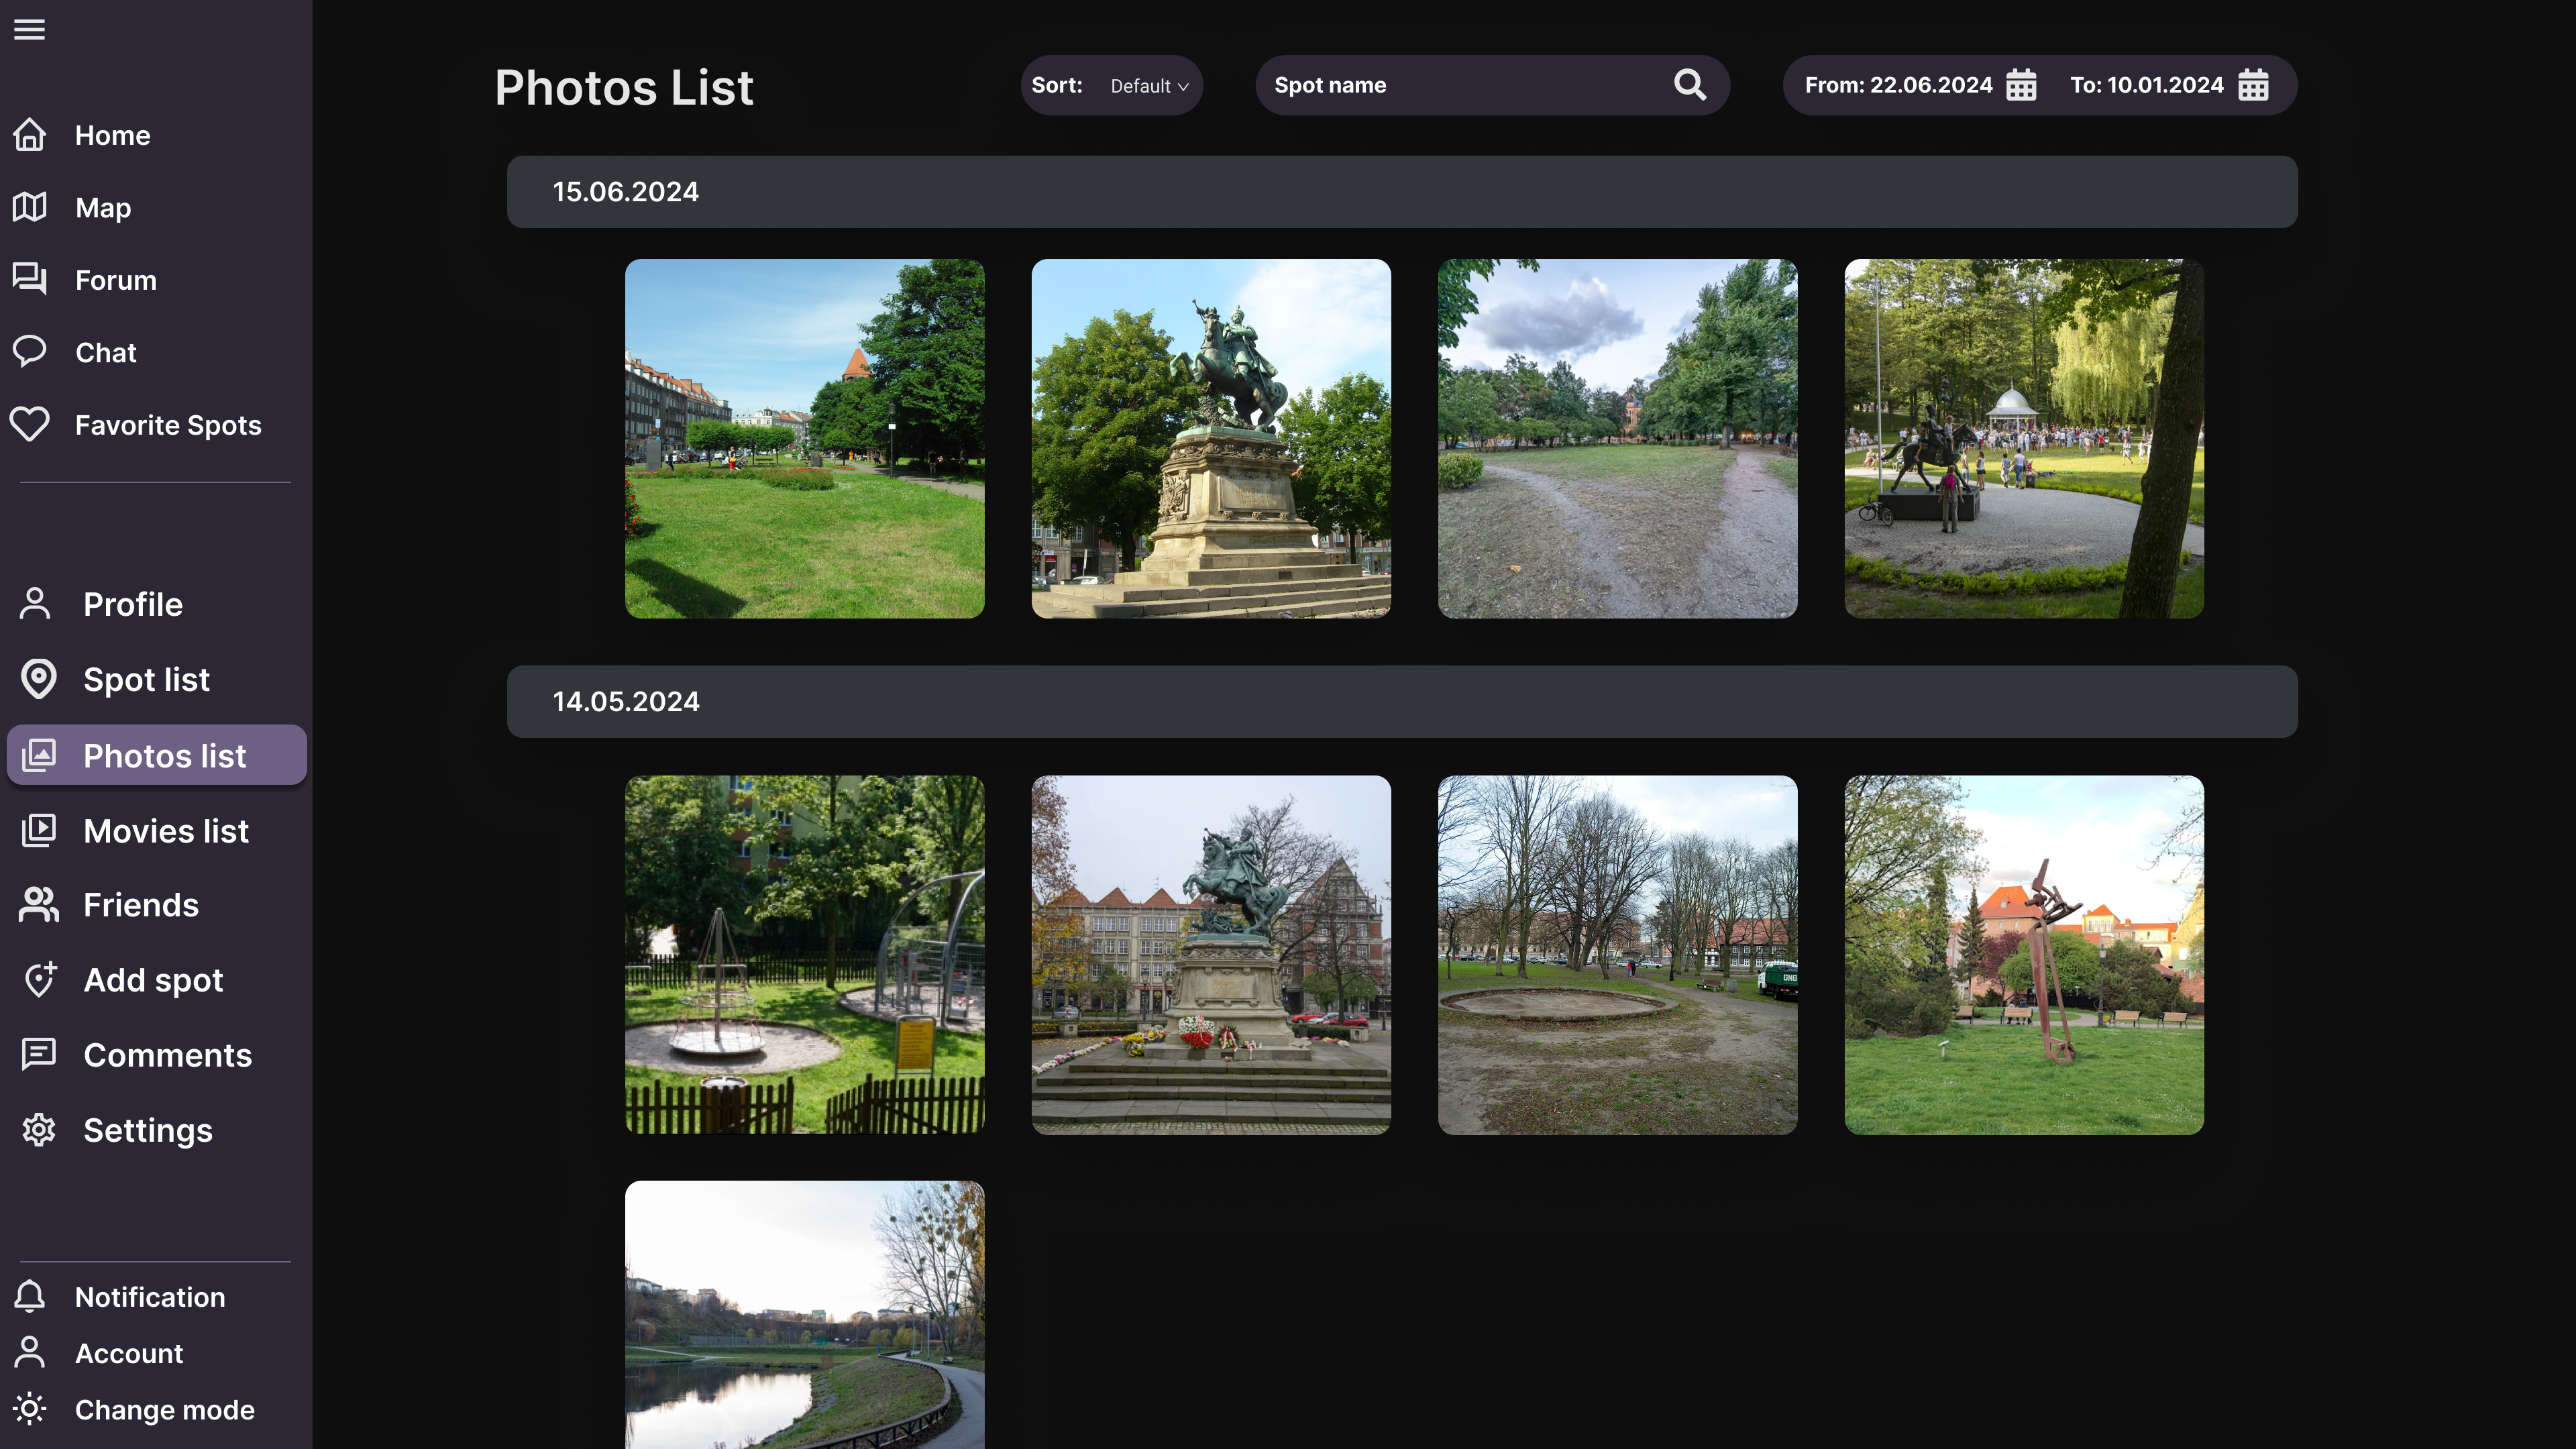
\includegraphics[width=1\textwidth]{attachments/prezentacja-systemu/panel-uzytkownika/photos}
    \caption{Lista zdjęć użytkownika.}
    \label{fig:photos}
\end{figure}

\begin{figure}[H]
    \centering
    \includegraphics[width=1\textwidth]{attachments/prezentacja-systemu/panel-uzytkownika/photos-empty}
    \caption{Komunikat pustego stanu w przypadku braku zdjęć.}
    \label{fig:photos-empty}
\end{figure}

Listę zdjęć można sortować oraz filtrować (rys. \ref{fig:photos-sort}).
Po ustawieniu parametrów lista jest odświeżana automatycznie (rys. \ref{fig:photos-filtered}).

\begin{figure}[H]
    \centering
    \includegraphics[width=1\textwidth]{attachments/prezentacja-systemu/panel-uzytkownika/photos-sort}
    \caption{Opcje sortowania i filtrowania listy zdjęć.}
    \label{fig:photos-sort}
\end{figure}

\begin{figure}[H]
    \centering
    \includegraphics[width=1\textwidth]{attachments/prezentacja-systemu/panel-uzytkownika/photos-filtered}
    \caption{Widok listy zdjęć po zastosowaniu filtrów/sortowania.}
    \label{fig:photos-filtered}
\end{figure}

Po najechaniu na zdjęcie wyświetlany jest przyciemniony pasek ze statystykami (analogicznie jak w profilu),
co pokazano na rys. \ref{fig:photos-hover}.
Dostępny jest również tryb ciemny (rys. \ref{fig:photos-dark}).

\begin{figure}[H]
    \centering
    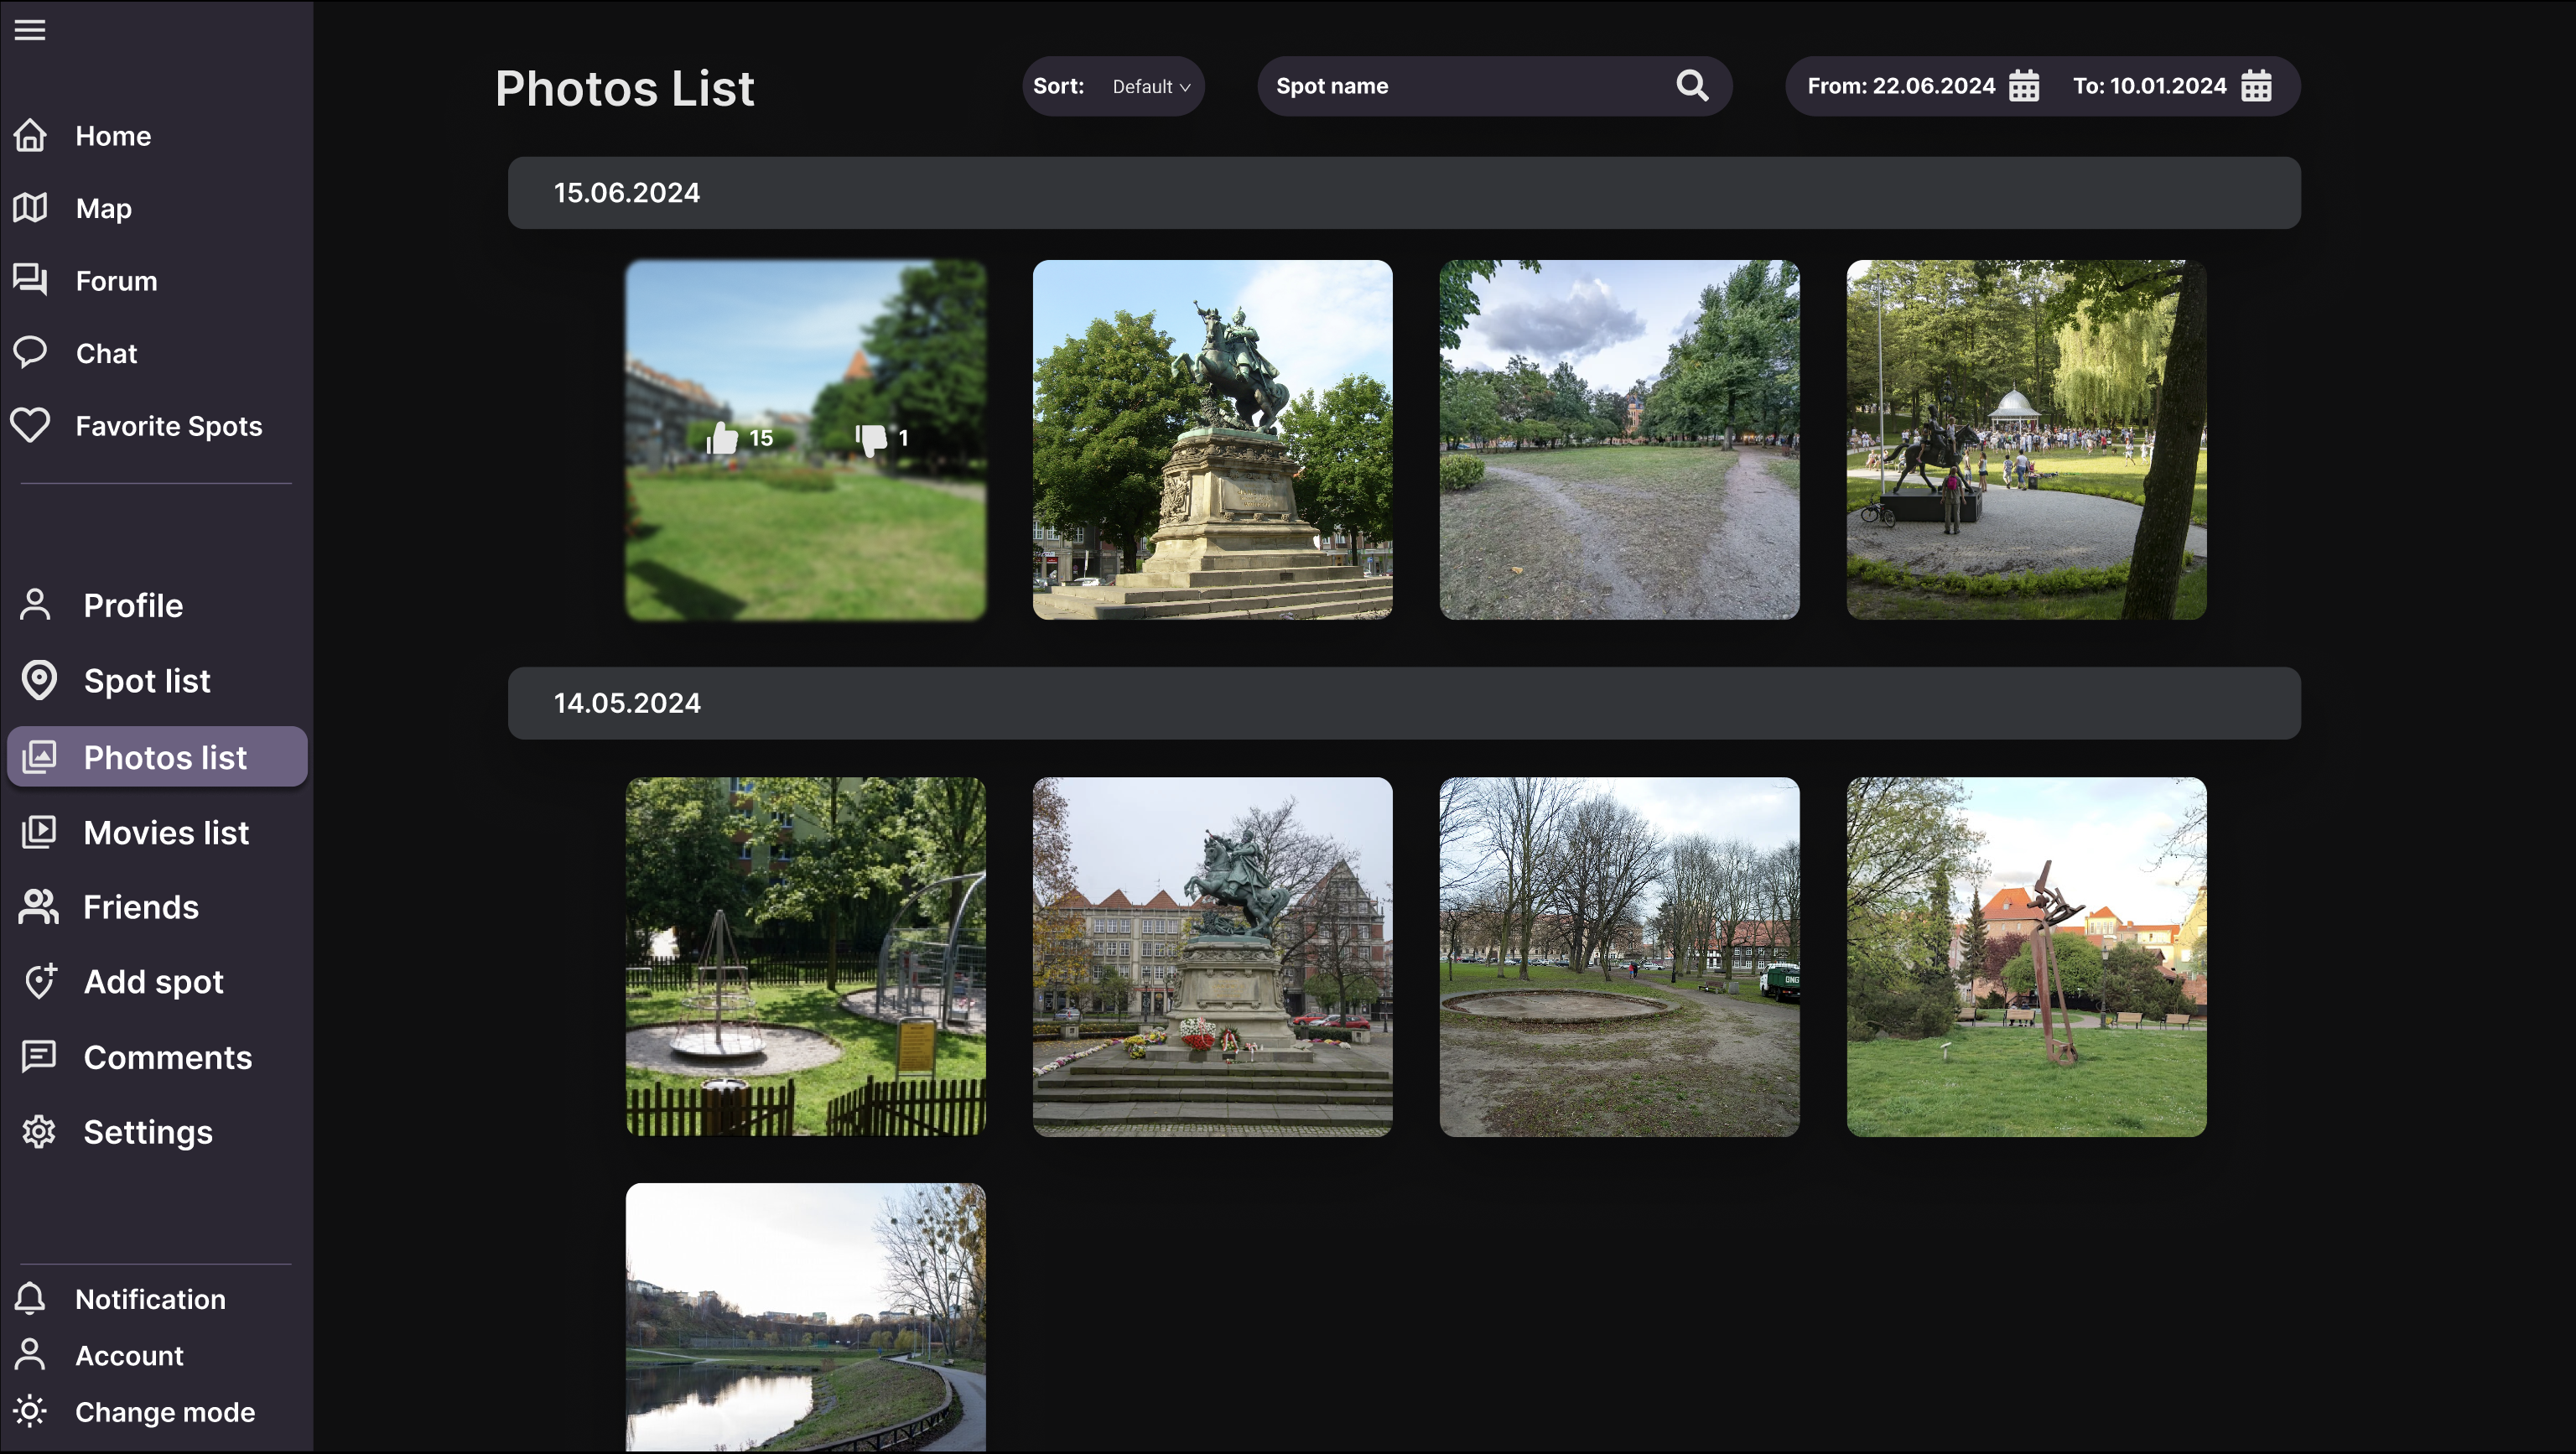
\includegraphics[width=1\textwidth]{attachments/prezentacja-systemu/panel-uzytkownika/photos-hover}
    \caption{Efekt najechania na kafelek zdjęcia (prezentacja statystyk).}
    \label{fig:photos-hover}
\end{figure}

\begin{figure}[H]
    \centering
    \includegraphics[width=1\textwidth]{attachments/prezentacja-systemu/panel-uzytkownika/photos-dark}
    \caption{Lista zdjęć w trybie ciemnym.}
    \label{fig:photos-dark}
\end{figure}

\subsubsection{Movies}

Sekcja \textit{Movies} prezentuje listę filmów dodanych przez użytkownika (rys. \ref{fig:movies}).
W przypadku braku filmów wyświetlany jest komunikat pustego stanu (rys. \ref{fig:movies-empty}).
Dostępne są analogiczne mechanizmy filtrowania i sortowania jak w sekcji \textit{Photos}.

\begin{figure}[H]
    \centering
    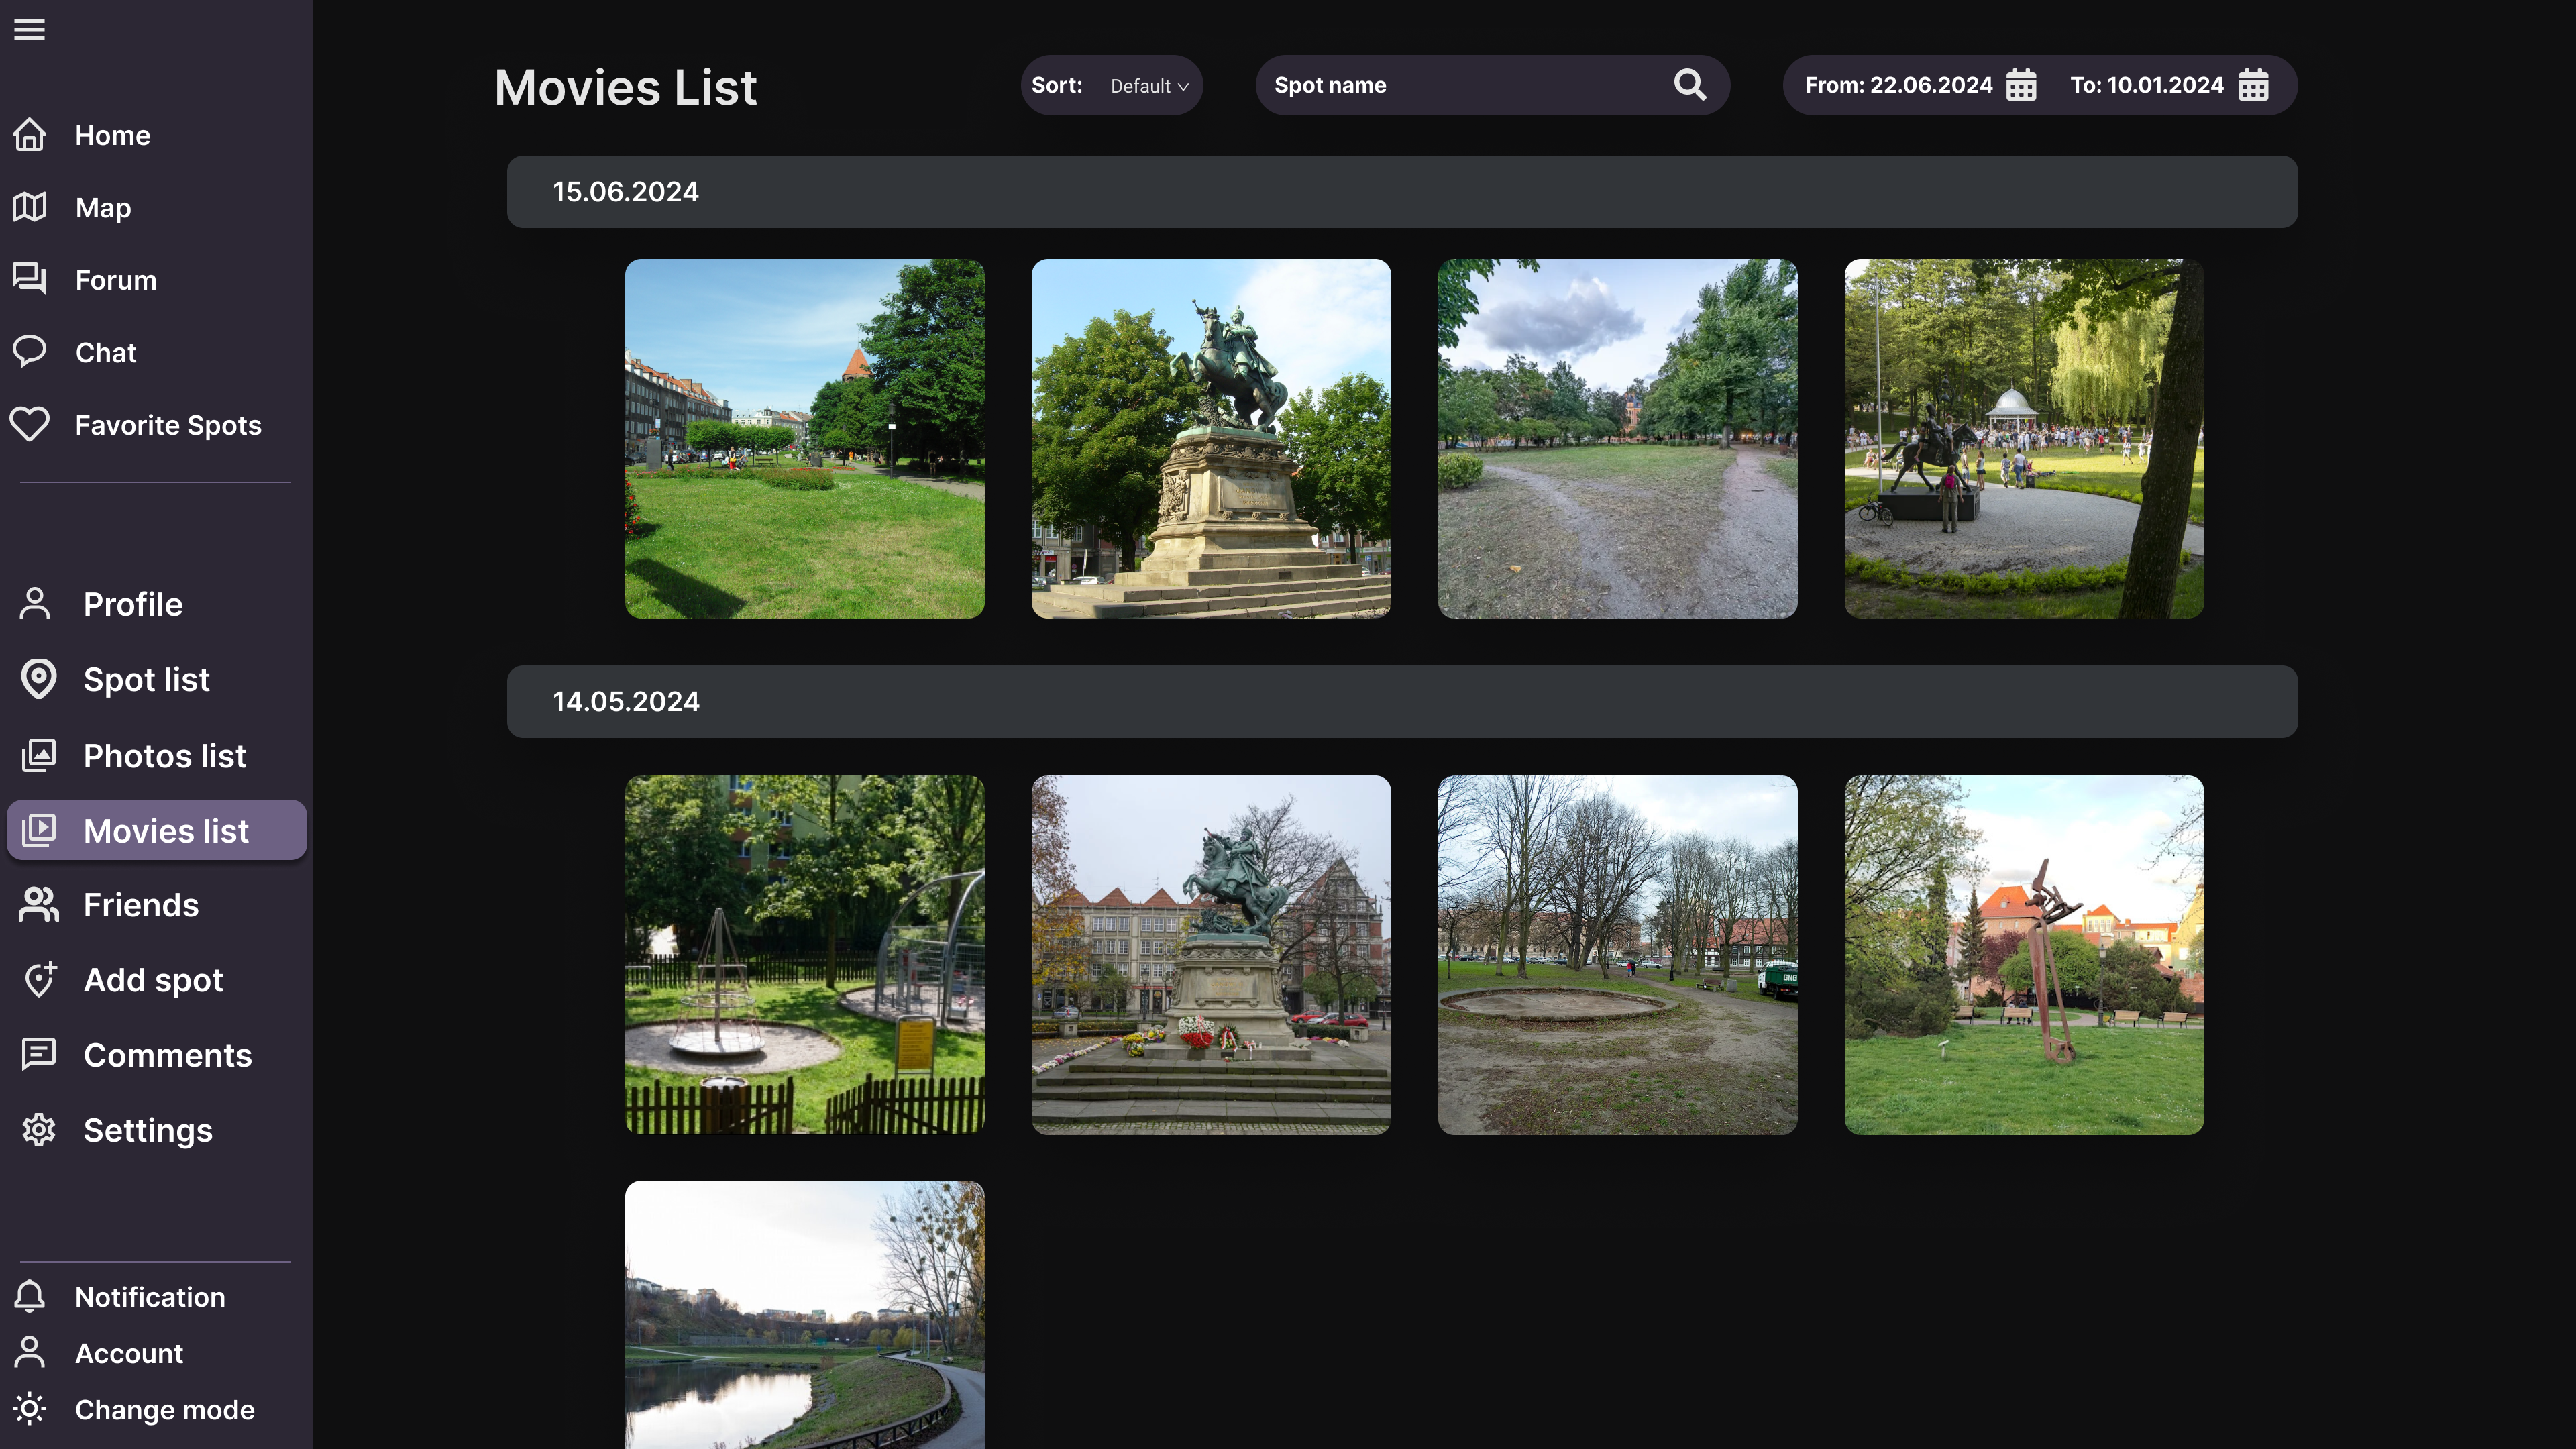
\includegraphics[width=1\textwidth]{attachments/prezentacja-systemu/panel-uzytkownika/movies}
    \caption{Lista filmów użytkownika.}
    \label{fig:movies}
\end{figure}

\begin{figure}[H]
    \centering
    \includegraphics[width=1\textwidth]{attachments/prezentacja-systemu/panel-uzytkownika/movies-empty}
    \caption{Komunikat pustego stanu w przypadku braku filmów.}
    \label{fig:movies-empty}
\end{figure}

Po najechaniu na kafelek filmu prezentowane są statystyki w przyciemnionym polu (rys. \ref{fig:movies-hover}).
Widok w trybie ciemnym pokazano na rys. \ref{fig:movies-dark}.

\begin{figure}[H]
    \centering
    \includegraphics[width=1\textwidth]{attachments/prezentacja-systemu/panel-uzytkownika/movies-hover}
    \caption{Efekt najechania na film (prezentacja statystyk).}
    \label{fig:movies-hover}
\end{figure}

\begin{figure}[H]
    \centering
    \includegraphics[width=1\textwidth]{attachments/prezentacja-systemu/panel-uzytkownika/movies-dark}
    \caption{Lista filmów w trybie ciemnym.}
    \label{fig:movies-dark}
\end{figure}

\subsubsection{Social}

Sekcja \textit{Social} udostępnia trzy listy: znajomych, obserwowanych oraz obserwujących
(rys. \ref{fig:social-friends}--\ref{fig:social-followers}).
Każdy kafelek użytkownika zawiera przyciski akcji (przejście do profilu, rozpoczęcie rozmowy, usunięcie).

\begin{figure}[H]
    \centering
    \includegraphics[width=1\textwidth]{attachments/prezentacja-systemu/panel-uzytkownika/social-friends}
    \caption{Zakładka \textit{Friends} w sekcji Social.}
    \label{fig:social-friends}
\end{figure}

\begin{figure}[H]
    \centering
    \includegraphics[width=1\textwidth]{attachments/prezentacja-systemu/panel-uzytkownika/social-followed}
    \caption{Zakładka \textit{Followed} w sekcji Social.}
    \label{fig:social-followed}
\end{figure}

\begin{figure}[H]
    \centering
    \includegraphics[width=1\textwidth]{attachments/prezentacja-systemu/panel-uzytkownika/social-followers}
    \caption{Zakładka \textit{Followers} w sekcji Social.}
    \label{fig:social-followers}
\end{figure}

Usunięcie znajomego wymaga potwierdzenia w oknie dialogowym (rys. \ref{fig:social-remove}).
Po zaakceptowaniu akcja jest wykonywana, a lista odświeżana (rys. \ref{fig:social-removed}).

\begin{figure}[H]
    \centering
    \includegraphics[width=1\textwidth]{attachments/prezentacja-systemu/panel-uzytkownika/social-remove}
    \caption{Okno potwierdzenia usunięcia użytkownika ze znajomych.}
    \label{fig:social-remove}
\end{figure}

\begin{figure}[H]
    \centering
    \includegraphics[width=1\textwidth]{attachments/prezentacja-systemu/panel-uzytkownika/social-removed}
    \caption{Lista znajomych po usunięciu wybranego użytkownika.}
    \label{fig:social-removed}
\end{figure}

Dodawanie nowych znajomych realizowane jest przez okno modalne z polem wyszukiwania po nazwie użytkownika
(rys.~\ref{fig:social-search}).
W trakcie wpisywania wyświetlana jest lista pasujących wyników (rys.~\ref{fig:social-search2}).
Po wysłaniu zaproszenia adresat widzi je w oknie zaproszeń dostępnym po kliknięciu przycisku
\textit{See friend invites} (rys.~\ref{fig:social-invites}).
Jeśli brak zaproszeń, prezentowany jest komunikat pustego stanu (rys.~\ref{fig:social-invites-empty}).

\begin{figure}[H]
    \centering
    \includegraphics[width=1\textwidth]{attachments/prezentacja-systemu/panel-uzytkownika/social-search}
    \caption{Okno wyszukiwania użytkownika podczas dodawania znajomego.}
    \label{fig:social-search}
\end{figure}

\begin{figure}[H]
    \centering
    \includegraphics[width=1\textwidth]{attachments/prezentacja-systemu/panel-uzytkownika/social-search2}
    \caption{Wyniki wyszukiwania użytkowników podczas dodawania znajomego.}
    \label{fig:social-search2}
\end{figure}

\begin{figure}[H]
    \centering
    \includegraphics[width=1\textwidth]{attachments/prezentacja-systemu/panel-uzytkownika/social-invites}
    \caption{Okno zaproszeń do znajomych z możliwością akceptacji/odrzucenia.}
    \label{fig:social-invites}
\end{figure}

\begin{figure}[H]
    \centering
    \includegraphics[width=1\textwidth]{attachments/prezentacja-systemu/panel-uzytkownika/social-invites-empty}
    \caption{Komunikat pustego stanu dla okna zaproszeń (brak zaproszeń).}
    \label{fig:social-invites-empty}
\end{figure}

W sekcji dostępny jest także tryb ciemny (rys.~\ref{fig:social-dark}).

\begin{figure}[H]
    \centering
    \includegraphics[width=1\textwidth]{attachments/prezentacja-systemu/panel-uzytkownika/social-dark}
    \caption{Sekcja Social w trybie ciemnym.}
    \label{fig:social-dark}
\end{figure}

\subsubsection{Add spot}

Sekcja \textit{Add spot} prezentuje listę \glslink{spot}{spotów} dodanych przez użytkownika do aplikacji (rys.~\ref{fig:add-spot-full}).
W przypadku braku wpisów wyświetlany jest komunikat pustego stanu (rys.~\ref{fig:add-spot-empty}).
W prawym górnym rogu dostępny jest przycisk \textit{Add Spot}, który otwiera formularz dodawania
nowego \glslink{spot}{spota} (rys.~\ref{fig:add-spot-form}).

\begin{figure}[H]
    \centering
    \includegraphics[width=1\textwidth]{attachments/prezentacja-systemu/panel-uzytkownika/add-spot-full}
    \caption{Lista spotów dodanych przez użytkownika do aplikacji.}
    \label{fig:add-spot-full}
\end{figure}

\begin{figure}[H]
    \centering
    \includegraphics[width=1\textwidth]{attachments/prezentacja-systemu/panel-uzytkownika/add-spot}
    \caption{Komunikat pustego stanu w sekcji Add spot (brak dodanych spotów).}
    \label{fig:add-spot-empty}
\end{figure}

\begin{figure}[H]
    \centering
    \includegraphics[width=1\textwidth]{attachments/prezentacja-systemu/panel-uzytkownika/add-spot-form}
    \caption{Formularz dodawania nowego spota.}
    \label{fig:add-spot-form}
\end{figure}

W formularzu zastosowano walidację danych.
W przypadku braku wymaganych informacji wyświetlane są komunikaty walidacyjne (rys.~\ref{fig:add-spot-error}).

\begin{figure}[H]
    \centering
    \includegraphics[width=1\textwidth]{attachments/prezentacja-systemu/panel-uzytkownika/add-spot-error}
    \caption{Walidacja formularza dodawania spota (komunikaty błędów).}
    \label{fig:add-spot-error}
\end{figure}

Dla załączonych miniatur zdjęć przewidziano interakcję usuwania: po najechaniu pojawia się przyciemnienie,
a kliknięcie powoduje usunięcie miniatury (rys.~\ref{fig:add-spot-hover}).
Widok w trybie ciemnym przedstawiono na rys.~\ref{fig:add-spot-dark}.

\begin{figure}[H]
    \centering
    \includegraphics[width=1\textwidth]{attachments/prezentacja-systemu/panel-uzytkownika/add-spot-hover}
    \caption{Interakcja usunięcia miniatury zdjęcia w formularzu (hover).}
    \label{fig:add-spot-hover}
\end{figure}

\begin{figure}[H]
    \centering
    \includegraphics[width=1\textwidth]{attachments/prezentacja-systemu/panel-uzytkownika/add-spot-dark}
    \caption{Sekcja Add spot w trybie ciemnym.}
    \label{fig:add-spot-dark}
\end{figure}

\subsubsection{Comments}

Sekcja \textit{Comments} prezentuje listę komentarzy dodanych przez użytkownika (rys.~\ref{fig:comments}).
Układ oraz sposób prezentacji nawiązuje do list zdjęć i filmów.
Jeśli brak komentarzy, wyświetlany jest komunikat pustego stanu (rys.~\ref{fig:comments-empty}).
Dostępny jest także tryb ciemny (rys.~\ref{fig:comments-dark}).

\begin{figure}[H]
    \centering
    \includegraphics[width=1\textwidth]{attachments/prezentacja-systemu/panel-uzytkownika/comments}
    \caption{Lista komentarzy użytkownika.}
    \label{fig:comments}
\end{figure}

\begin{figure}[H]
    \centering
    \includegraphics[width=1\textwidth]{attachments/prezentacja-systemu/panel-uzytkownika/comments-empty}
    \caption{Komunikat pustego stanu w sekcji Comments (brak komentarzy).}
    \label{fig:comments-empty}
\end{figure}

\begin{figure}[H]
    \centering
    \includegraphics[width=1\textwidth]{attachments/prezentacja-systemu/panel-uzytkownika/comments-dark}
    \caption{Sekcja Comments w trybie ciemnym.}
    \label{fig:comments-dark}
\end{figure}

\subsubsection{Settings}

Ostatnią sekcją są ustawienia konta.
Prezentowane są podstawowe dane (nazwa użytkownika, e-mail, hasło) wraz z przyciskami \textit{Edit} (rys.~\ref{fig:settings}).
Po wybraniu edycji w prawym obszarze widoku pojawia się odpowiedni formularz zmiany danych: nazwy
użytkownika (rys.~\ref{fig:settings-username}), adresu e-mail (rys.~\ref{fig:settings-email}) lub
hasła (rys.~\ref{fig:settings-password}). W przypadku hasła przewidziano pola na stare hasło,
nowe hasło oraz potwierdzenie.

\begin{figure}[H]
    \centering
    \includegraphics[width=1\textwidth]{attachments/prezentacja-systemu/panel-uzytkownika/settings}
    \caption{Widok ustawień konta (Account details).}
    \label{fig:settings}
\end{figure}

\begin{figure}[H]
    \centering
    \includegraphics[width=1\textwidth]{attachments/prezentacja-systemu/panel-uzytkownika/settings-username}
    \caption{Formularz zmiany nazwy użytkownika.}
    \label{fig:settings-username}
\end{figure}

\begin{figure}[H]
    \centering
    \includegraphics[width=1\textwidth]{attachments/prezentacja-systemu/panel-uzytkownika/settings-email}
    \caption{Formularz zmiany adresu e-mail.}
    \label{fig:settings-email}
\end{figure}

\begin{figure}[H]
    \centering
    \includegraphics[width=1\textwidth]{attachments/prezentacja-systemu/panel-uzytkownika/settings-password}
    \caption{Formularz zmiany hasła (stare hasło, nowe hasło, potwierdzenie).}
    \label{fig:settings-password}
\end{figure}

Dla ustawień przygotowano również wariant ciemny (rys.~\ref{fig:settings-dark}), w którym dostosowano kontrast
pól formularzy i elementów nawigacji.

\begin{figure}[H]
    \centering
    \includegraphics[width=1\textwidth]{attachments/prezentacja-systemu/panel-uzytkownika/settings-dark}
    \caption{Ustawienia konta w trybie ciemnym.}
    \label{fig:settings-dark}
\end{figure}

